\chapter{低层视觉处理:视网膜} \label{chap:chap22}

视网膜是大脑观察世界的窗口。
所有的\textit{视觉经验}都基于眼睛中这个神经回路处理信息。
视网膜的输出仅通过一百万个视神经纤维传送到大脑,但几乎一半的大脑皮层用于处理这些信号。
由于设计或缺陷而丢失在视网膜中的视觉信息永远无法恢复。
由于视网膜处理对可以看到的内容设置了基本限制,因此人们对了解视网膜的功能非常感兴趣。


从表面上看,脊椎动物的眼睛看起来很像相机。
如图~\ref{fig:22_1}~所示,瞳孔形成可变孔径,角膜和晶状体提供折射光学器件,将外部世界的小图像投射到眼球后部的光敏视网膜上。
但这就是眼睛和相机类比结束的地方。
如图~\ref{fig:22_2}~所示,视网膜是一层薄薄的神经元,厚几百微米,由 5 种主要细胞类型组成,这些细胞排列在由 2 个突触层隔开的 3 个细胞层中。


\begin{figure}[htbp]
	\centering
	\includegraphics[width=1.0\linewidth]{chap22/fig_22_1}
	\caption{眼睛将视觉场景投射到视网膜的感光器上。
		A. 来自视野中物体的光被角膜和晶状体折射并聚焦到视网膜上。
		B. 在中央凹,对应于凝视的正中心,视网膜的近端神经元被移到一边,因此光线可以直接进入光受体。
		C. 用于评估正常视力的视力表中的字母被投射到中央凹中密集的光受体上。
		由于肉眼的光学衍射,虽然不像这里显示的那样清晰,但字母的最小可辨别笔画宽度约为一个视锥细胞直径\cite{curcio1991organization}。}
	\label{fig:22_1}
\end{figure}


\begin{figure}[htbp]
	\centering
	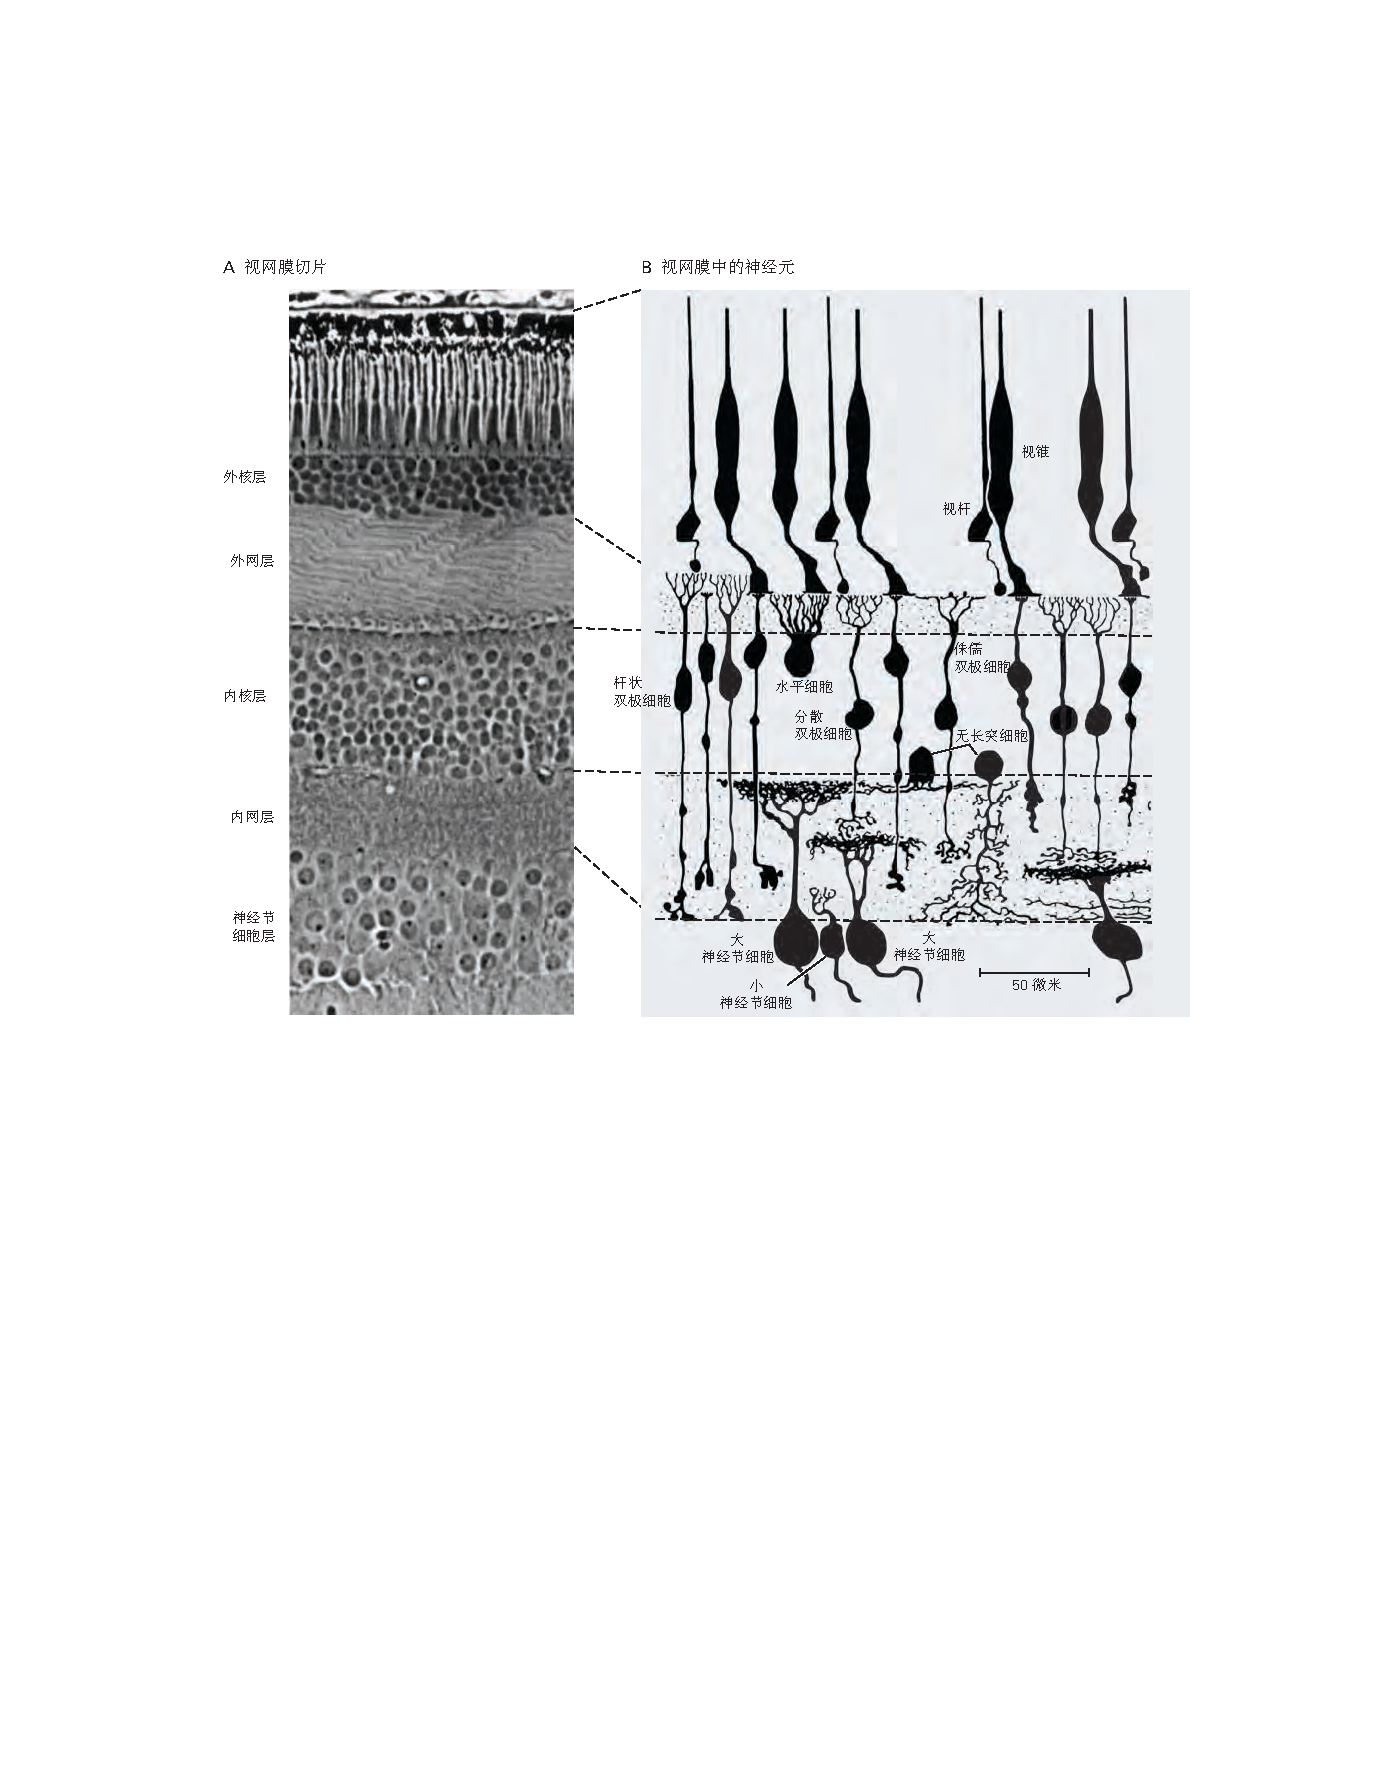
\includegraphics[width=1.0\linewidth]{chap22/fig_22_2}
	\caption{视网膜包括 5 个不同的神经元和突触层。
		A. 通过光学显微镜看到的人类视网膜的垂直截面。
		3 层细胞体明显。
		外核层包含感光细胞体;内核层包括水平细胞、双极细胞和无长突细胞;神经节细胞层含有神经节细胞和一些移位的无长突细胞。
		2 层纤维和突触将它们分开:\textit{外网层}和\textit{内网层}~\cite{boycott1969organization}。
		B. 基于高尔基体染色的猕猴视网膜神经元。
		细胞层和突触层与 A 部分中的图像对齐\cite{polyak1941retina}。}
	\label{fig:22_2}
\end{figure}


最外层的感光细胞吸收光并将其转化为神经信号,这一过程称为光转导。
这些信号通过突触传递到双极细胞,双极细胞又连接到最内层的视网膜神经节细胞。
视网膜神经节细胞是视网膜的输出神经元,它们的轴突形成视神经。
如图~\ref{fig:22_3}~所示,除了从感觉神经元到输出神经元的这种直接通路外,视网膜回路还包括许多由外部突触层中的水平细胞和内部突触层中的无长突细胞提供的横向连接。


\begin{figure}[htbp]
	\centering
	\includegraphics[width=1.0\linewidth]{chap22/fig_22_3}
	\caption{视网膜回路。
		A. 视锥信号的回路,显示分裂成\textit{给光细胞}通路和\textit{撤光细胞}通路(参见图~\ref{fig:22_10})以及外层\textit{侧抑制}通路。
		红色箭头表示通过电突触或谷氨酸能突触的信号保持连接。
		灰色箭头表示通过\textit{$\gamma-$氨基丁酸能突触}、\textit{甘氨酸能突触}或\textit{谷氨酸能突触}的符号反转连接。
		B. 视杆信号通过 AII 无长突细胞进入视锥回路,\textit{给光细胞}通路和\textit{撤光细胞}通路在此处分开。}
	\label{fig:22_3}
\end{figure}
% AII 无长突细胞 是 视网膜中的无长突细胞的一个亚型


视网膜回路执行低层视觉处理,这是视觉图像分析的初始阶段。
它从眼睛的原始图像中提取某些空间和时间特征,并将它们传送到更高的视觉中心。
这种处理的规则适应环境条件的变化。
特别是,视网膜必须调整其对不断变化的照明条件的敏感度。
尽管在每天的过程中遇到的光强度范围很大,但这种适应使我们的视力或多或少保持稳定。


在本章中,我们依次讨论了视网膜功能的 3 个重要方面:光转导、预处理和适应。
我们将说明实现它们的神经机制及其对视觉感知的影响。



\section{光感层对视觉图像进行采样}

\subsection{眼光学限制了视网膜图像的质量}

视网膜图像的清晰度由几个因素决定:
瞳孔孔径处的衍射、角膜和晶状体的屈光不正以及光路中材料引起的散射。
外界的一个点通常会聚焦在视网膜上一个模糊的小圆圈中。
与其他光学设备一样,这种模糊在光轴附近最小,图像质量接近光瞳衍射所施加的极限。
远离轴时,由于角膜和晶状体的像差,图像会显著退化,并且可能会因光散射白内障或近视等屈光不正等异常情况而进一步退化。


靠近光轴的视网膜区域(中央凹)是视力最敏锐的地方,对应于指向我们关注物体的注视中心。
如图~\ref{fig:22_1}B~所示,感光细胞、双极细胞和神经节细胞的密度在中央凹处最高。
感光器之间的间距与光学模糊圈的大小非常匹配,因此以理想的方式对图像进行采样。
如图~\ref{fig:22_1}B~所示,光在到达感光器之前通常必须穿过几层细胞,但在称为中央凹的中心,其他细胞层被推到一边以减少光散射造成的额外模糊。
最后,眼睛后部盖着一层黑色色素上皮,它吸收光线并防止光线散射回眼睛。


如图~\ref{fig:22_1}A~所示,视网膜包含另一个特殊部位(即视盘),视网膜神经节细胞的轴突汇聚并延伸穿过视网膜,从眼睛后部出现,成为视神经。
必然地,该区域没有光受体,因此对应于每只眼睛视野中的盲点。
由于圆盘位于每只眼睛的中央凹的鼻侧,来自 1 个点的光不会同时落在 2 个盲点上,因此通常我们不会注意到它们。
如图~\ref{fig:22_4}~所示,我们可以只用一只眼睛体验盲点。
盲点展示了盲人的体验(不是黑暗,而是什么都没有)。
这就解释了为什么周围视网膜的损伤经常被忽视。
通常是由于意外事故,例如撞到未引起注意的物体,或通过临床测试发现视力缺陷。


\begin{figure}[htbp]
	\centering
	\includegraphics[width=0.7\linewidth]{chap22/fig_22_4}
	\caption{人类视网膜的盲点。
		通过闭上右眼并用左眼固定十字来定位左眼的盲点。
		将书拿在离眼睛大约 30 厘米的地方,然后将其稍微靠近或远离,直到左边的圆圈消失。
		现在将一支铅笔垂直放在页面上,然后将它从侧面扫过圆圈。 
		请注意,尽管没有光线可以从圆圈区域到达您的视网膜,但铅笔似乎没有折断。 
		接下来,纵向移动铅笔,观察当它的笔尖进入圆圈时会发生什么\cite{hurvich1981color}。}
	\label{fig:22_4}
\end{figure}


盲点是视网膜由内而外设计的必然结果,这让几代生物学家感到困惑和好笑。
该组织的目的可能是使光受体与视网膜色素上皮细胞紧密并置,这在视网膜色素更新和通过吞噬作用回收光受体膜中起着重要作用。


\subsection{有 2 种类型的光受体:视杆细胞和视锥细胞}

如图~\ref{fig:22_5}A~所示,所有的感光细胞都有一个共同的结构,有 4 个功能区域:
外段(位于神经视网膜的远端表面)、
内段(位于更近端)、细胞体和\textit{突触末稍}。


\begin{figure}[htbp]
	\centering
	\includegraphics[width=1.0\linewidth]{chap22/fig_22_5}
	\caption{\textit{视杆光受体}和\textit{视锥光感光器}具有相似的结构。
		A. 视杆细胞和视锥细胞都有称为\textit{外段}和\textit{内段}的特殊区域。
		\textit{外段}通过\textit{纤毛}连接到\textit{内段}并包含光转换装置。
		内部部分包含线粒体和许多蛋白质合成机器。
		B. \textit{外段}由一堆含有吸光感光色素的\textit{膜盘}组成。
		在这 2 种类型的细胞中,这些圆盘都是通过\textit{细胞质膜}的折叠形成。
		然而,在杆状细胞中,褶皱从膜上夹断,因此圆盘在\textit{外段}内自由漂浮,而在视锥细胞中,圆盘仍然是\textit{细胞质膜}的一部分\cite{o1982chemistry,young1970visual}。}
	\label{fig:22_5}
\end{figure}


大多数脊椎动物有 2 种类型的光受体(即视杆细胞和视锥细胞),以它们的形态来区分。
如图~\ref{fig:22_5}B~所示,视杆细胞有一个长的圆柱形外段,其中圆盘堆叠与细胞质膜分开,而视锥细胞通常有一个较短的视锥细胞外段,圆盘与外膜连续。


视杆细胞和视锥细胞在功能上也有所不同,最重要的是它们对光的敏感性。
视杆细胞可以发出吸收单个光子的信号,并负责在月光等昏暗光照下的视觉。
但是随着接近黎明的光照水平增加,杆状细胞的电响应变得饱和,细胞停止对强度变化做出响应。
视锥细胞对光的敏感度要低得多;
它们对夜视没有贡献,但只负责白天的视力。
它们的响应比视杆细胞快得多。
如图~\ref{fig:22_6}~所示,灵长类动物只有一种视杆细胞,但有 3 种视锥细胞光受体,根据它们响应的波长范围来区分:长波视锥细胞、\textit{中波}视锥细胞和\textit{短波}视锥细胞。


人类视网膜包含大约 1 亿个视杆细胞和 500 万个视锥细胞,但这 2 种细胞类型的分布不同。
中央凹不包含视杆细胞,但密集地排列着小视锥细胞。
在中央凹外几毫米处,视杆细胞的数量远远多于视锥细胞。
所有的光受体都变得更大,并向视网膜周边分布得更广。
\textit{短波}视锥细胞仅占所有视锥细胞的 10\%,并且不存在于中央凹中。


视网膜注视中心显然专用于白天视觉。
中央凹中视锥细胞光受体的密集堆积设定了我们视力的极限。
事实上,如图~\ref{fig:22_1}C~所示,我们可以在医生的视力表上读到的最小字母具有笔画,其图像在视网膜上只有 1 到 2 个视锥细胞直径宽,视角约为 1 分弧。
到了晚上,由于没有视杆细胞,中央凹是盲的。
天文学家知道,必须只看一颗昏暗恒星的侧面才能看到它。
夜间在森林里散步时,我们这些非天文学家往往会跟随白天的反射,直视可疑声音的来源。 
神秘的是,这个物体消失了,只是在我们移开视线时跳回了我们的周边视野。



\section{光转导将光子的吸收与膜电导的变化联系起来}

与许多其他神经元一样,光受体的膜电位受膜电导与~\ce{Na+} 和~\ce{K+} 平衡的调节,其跨膜梯度由代谢活性泵维持(第~\ref{chap:chap9}~章)。
在黑暗中,\ce{Na+} 通过非选择性阳离子通道流入光受体,该通道由第二信使\textit{环鸟苷-3,5-单磷酸盐}激活。


色素蛋白对光子的吸收启动了生化级联响应,最终降低了\textit{环鸟苷-3,5-单磷酸盐}的浓度,从而关闭了\textit{环鸟苷-3,5-单磷酸盐}门控通道,使细胞更接近~\ce{K+}平衡电位。
如图~\ref{fig:22_7}~所示,通过这种方式,光使感光器超极化。
在这里,我们详细描述了这一系列事件。
这些知识大部分来自对杆状细胞的研究,但视锥细胞中的机制非常相似。


\begin{figure}[htbp]
	\centering
	\includegraphics[width=1.0\linewidth]{chap22/fig_22_7}
	\caption{光转导。
		A. 视杆细胞对光有响应。
		\textit{外段}视盘中的视紫红质分子吸收光子,导致\textit{细胞质膜}中\textit{环鸟苷-3,5-单磷酸盐}门控通道关闭。
		这种通道关闭使膜超极化并降低神经递质谷氨酸的释放速率\cite{alberts2017molecular}。
		B. 1. 光转导中的分子过程。
		\textit{环鸟苷-3,5-单磷酸盐}由\textit{鸟苷酸环化酶}从\textit{三磷酸鸟苷}产生并被\textit{磷酸二酯酶}水解。
		在黑暗中,磷酸二酯酶活性低,\textit{环鸟苷-3,5-单磷酸盐}浓度高,\textit{环鸟苷-3,5-单磷酸盐}门控通道开放,允许 \ce{Na+} 和 \ce{Ca^2+} 流入。
		在光线下,\textit{视紫红质}通过吸收光子而被激发,然后激活\textit{转导蛋白},\textit{转导蛋白}进而激活\textit{磷酸二酯酶};
		\textit{环鸟苷-3,5-单磷酸盐}水平下降,膜通道关闭,更少的 \ce{Na+} 和 \ce{Ca^2+} 进入细胞。
		转导酶均位于内膜圆盘中,可溶性配体\textit{环鸟苷-3,5-单磷酸盐}作为细胞质膜的信使。
		2. \ce{Ca^2+} 在光转导响应级联中具有负反馈作用。
		光对网络的刺激导致\textit{环鸟苷-3,5-单磷酸盐}门控通道的关闭。
		这导致细胞内 \ce{Ca^2+} 浓度下降。
		因为 \ce{Ca^2+} 调节至少 3 个级联组分的功能(视紫红质、\textit{鸟苷酸环化酶}和\textit{环鸟苷-3,5-单磷酸盐}门控通道)\ce{Ca^2+} 的下降抵消了光引起的激发。
		C. 灵长类视杆细胞和视锥细胞对强度增加的短暂闪光的电压响应。
		迹线上的数字越高表示光照强度越大(并非所有迹线都已标记)。 
		对于昏暗的闪光,响应幅度随强度线性增加。 
		在高强度下,受体饱和并在闪光后的一段时间内稳定地保持超极化;
		这会导致我们在明亮的闪光后看到的残像。 
		请注意,对于更亮的闪光,响应峰值更早,并且视锥细胞的响应速度比视杆细胞快\cite{schneeweis1995photovoltage}。}
	\label{fig:22_7}
\end{figure}



\subsection{光激活光受体中的色素分子}

视紫红质是视杆细胞中的视觉色素,有 2 种成分。
蛋白质部分视蛋白嵌入椎间视盘膜中,本身不吸收可见光。
如图~\ref{fig:22_8}A~所示,吸光部分(视黄醛)是一种小分子,其 11-顺式异构体与视蛋白的赖氨酸残基共价连接。
视网膜对光子的吸收导致它从 11-顺式构型翻转到全反式构型。
这种响应是视觉中唯一依赖光的步骤。


\begin{figure}[htbp]
	\centering
	\includegraphics[width=1.0\linewidth]{chap22/fig_22_8}
	\caption{视觉色素的结构。
		A. 视杆细胞中的视色素视紫红质是 2 种成分的共价复合物。
		视蛋白是一种大型蛋白质,具有 348 个氨基酸,分子量约为 4 万道尔顿。
		它在视杆细胞的膜上来回循环 7 次。
		视黄醛是一种小的吸光化合物,共价连接到视蛋白第 7 个跨膜区域赖氨酸 296 的侧链上。
		11-顺式视黄醛对光的吸收导致围绕双键的旋转。
		由于视网膜采用更稳定的全反式构型,它会引起视蛋白的构象变化,从而触发后续的视觉转导事件\cite{nathans1984isolation}。
		B. 蓝色圆圈表示相同的氨基酸;
		黑色圆圈表示差异。
		3 种视锥细胞(\textit{长波}、\textit{中波}和\textit{短波}中的视蛋白形式彼此相似,视杆细胞中的视紫红质也相似,这表明这 4 种细胞都是通过复制和发散从一个共同的前体进化而来的。
		\textit{长波}和\textit{中波}视蛋白的关系最为密切,其氨基酸序列具有 96\% 的同一性。
		它们被认为是从大约 3 千万年前的一次基因复制事件中进化而来的,当时\textit{旧大陆猴}具有 3 种视觉色素,而\textit{新大陆猴}通常只有 2 种。}
	\label{fig:22_8}
\end{figure}


视网膜分子形状的变化导致视蛋白的构象变化为激活状态(称为变视紫红质 II),从而触发光转导的第二步。
变视紫红质 II 不稳定,会在几分钟内分裂,产生视蛋白和游离的\textit{全反式视黄醛}。
然后全反式视黄醛从视杆细胞运送到色素上皮细胞,在那里它被还原为全反式视黄醇(维生素 A),即 11-顺式视黄醛的前体,随后被运回视杆细胞。


因此,\textit{全反式视黄醛}是视觉系统中的重要化合物。
它的前体(如维生素 A)不能由人类合成,因此必须作为日常饮食的一部分。
维生素 A 缺乏会导致夜盲症,如果不加以治疗,还会导致受体外段的退化并最终导致失明。


人类视网膜中的每种视锥细胞都会产生一种视蛋白变体。 
如图~\ref{fig:22_6}~所示,这 3 种视锥细胞色素的区别在于它们的吸收光谱,即光吸收效率对波长的依赖性。
光谱由蛋白质序列通过结合口袋附近的视黄醛和某些氨基酸侧链之间的相互作用来确定。
红光比\textit{中波}视锥细胞更能激发\textit{长波}视锥细胞,而绿光更能激发\textit{中波}视锥细胞。
因此,这些视锥细胞类型中的相对激发度包含有关光的光谱信息,与其强度无关。
大脑对来自不同视锥细胞类型的信号进行比较是色觉的基础。


\begin{figure}[htbp]
	\centering
	\includegraphics[width=0.55\linewidth]{chap22/fig_22_6}
	\caption{3 种视锥细胞和视杆细胞的灵敏度光谱。
		在每个波长下,灵敏度与在感觉神经元中引起标准响应所需的光强度成反比。 
		灵敏度在很大范围内变化,因此以对数刻度显示。 
		不同类别的光受体对广泛且重叠的波长范围敏感。}
	\label{fig:22_6}
\end{figure}


在夜视中,只有视杆细胞处于活动状态,因此所有功能性光受体都具有相同的吸收光谱。
因此,绿光对视觉系统的影响与强度更高的红光完全相同。
因为单光受体系统无法区分光的光谱和强度,所以“晚上所有的猫都是灰色的”。
通过比较视杆细胞对不同波长光的敏感度,可以获得视紫红质的吸收光谱。
如图~\ref{fig:22_9}~所示,一个了不起的事实是,只需向人类受试者询问各种彩色光的外观,就可以准确地测量这种分子特性。
知觉或心理物理学的定量研究为大脑处理的其他机制提供了类似的见解(第~\ref{chap:chap17}~章)。


\begin{figure}[htbp]
	\centering
	\includegraphics[width=0.8\linewidth]{chap22/fig_22_9}
	\caption{视紫红质的吸收光谱。
		将在试管中测量的人类视紫红质的吸收光谱与人类观察者对非常暗淡的闪光的光谱灵敏度进行比较。
		心理物理数据已针对眼部介质的吸收进行了校正。}
	\label{fig:22_9}
\end{figure}



\subsection{兴奋的视紫红质通过 G 蛋白转导蛋白激活磷酸二酯酶}

活化的视紫红质以变视紫红质 II 的形式扩散到视盘膜内,在那里它遇到转导蛋白,G 蛋白家族的一员(第~\ref{chap:chap14}~章)。
与其他 G 蛋白的情况一样,无活性形式的转导蛋白结合\textit{二磷酸鸟苷}分子。
与\textit{变视紫红质 II}的相互作用促进\textit{二磷酸鸟苷}与\textit{三磷酸鸟苷}的交换。
这导致转导蛋白的亚基解离为携带\textit{三磷酸鸟苷}(T$\alpha$-\textit{三磷酸鸟苷})以及$\beta$和$\gamma$亚基(T$\beta$$\gamma$)的活性$\alpha$亚基。
变视紫红质 II 可以激活数百个额外的转导蛋白分子,从而显著增强细胞的响应。


活性转导蛋白亚基 T$\alpha$-\textit{三磷酸鸟苷} 与环核苷酸磷酸二酯酶(另一种与椎间盘膜相关的蛋白质)形成复合物。
这种相互作用大大提高了酶将\textit{环鸟苷-3,5-单磷酸盐}水解为 5'-\textit{鸟苷-3,5-单磷酸盐}的速率。
每个磷酸二酯酶分子每秒可水解 1 千多个\textit{环鸟苷-3,5-单磷酸盐}分子,从而增加放大程度。


\textit{环鸟苷-3,5-单磷酸盐}的浓度控制外段细胞质膜中\textit{环鸟苷-3,5-单磷酸盐}门控通道的活性。
在黑暗中,当\textit{环鸟苷-3,5-单磷酸盐}浓度高时,大量 \ce{Na+} 通过开放通道流入,使细胞保持在大约 –40 毫伏的去极化水平。
结果,细胞的\textit{突触末稍}不断释放谷氨酸递质。
如图~\ref{fig:22_7}B1~所示,光诱发的\textit{环鸟苷-3,5-单磷酸盐}减少导致\textit{环鸟苷-3,5-单磷酸盐}门控通道关闭,从而减少 \ce{Na+} 的内流并使细胞超极化。
超极化减缓了光受体末端神经递质的释放,从而启动了神经信号。



\subsection{多重机制关断级联}

感光器对单个光子的响应必须终止,这样细胞才能对另一个光子做出响应。
通过特定的视紫红质激酶对视紫红质 II 进行磷酸化,然后结合可溶性蛋白抑制蛋白,从而阻断与转导蛋白的相互作用。


活性转导蛋白(T$\alpha$-\textit{三磷酸鸟苷})具有内在的\textit{三磷酸鸟苷}酶活性,最终将结合的\textit{三磷酸鸟苷}转化为\textit{二磷酸鸟苷}。
然后 T$\alpha$-\textit{二磷酸鸟苷}释放磷酸二酯酶并与 T$\beta$$\gamma$ 重组,再次准备好被视紫红质激发。
一旦磷酸二酯酶失活,\textit{环鸟苷-3,5-单磷酸盐}浓度就会通过从\textit{三磷酸鸟苷}产生\textit{环鸟苷-3,5-单磷酸盐}的鸟苷酸环化酶恢复。
此时,膜通道打开,\ce{Na+} 电流恢复,光受体去极化回到其暗电位。


除了这些关闭级联的各个元素的独立机制之外,重要的反馈机制可确保更快地终止大量响应。
这是由细胞中 \ce{Ca^2+} 浓度的变化介导的。
\ce{Ca^2+}通过\textit{环鸟苷-3,5-单磷酸盐}门控通道进入细胞,并被快速阳离子交换剂排出。
在黑暗中,细胞内 \ce{Ca^2+} 浓度较高,但在细胞对光响应期间,当\textit{环鸟苷-3,5-单磷酸盐}门控通道关闭时,\ce{Ca^2+} 水平迅速下降至黑暗水平的百分之几。


如图~\ref{fig:22_7}B2~所示,\ce{Ca^2+} 浓度的降低以 3 种方式调节生化响应。
钙结合蛋白恢复素对视紫红质激酶的作用可加速视紫红质磷酸化,从而减少转导蛋白的激活。
钙依赖性鸟苷酸环化酶激活蛋白可加速鸟苷酸环化酶的活性。
最后,\textit{环鸟苷-3,5-单磷酸盐}门控通道对\textit{环鸟苷-3,5-单磷酸盐}的亲和力通过 \ce{Ca^2+}-钙调蛋白的作用而增加。
所有这些作用促进光受体返回到黑暗状态。



\subsection{光转导缺陷导致疾病}

毫不奇怪,光转导机制中的缺陷会产生严重的后果。
一个突出的缺陷是色盲,这是由于视锥细胞色素基因缺失或异常引起的,稍后将对此进行讨论。


当视杆细胞功能丧失但视锥细胞功能保持完好时,就会导致静止性夜盲症。
这种疾病是可遗传的,并且已经在光转导级联的许多组分中发现了突变:视紫红质、杆状转导蛋白、杆状磷酸二酯酶、视紫红质激酶和抑制蛋白。
在某些情况下,视杆细胞似乎会永久激活,就好像暴露在持续的致盲光下一样。


不幸的是,许多光转导缺陷会导致色素性视网膜炎,这是一种视网膜进行性退化,最终导致失明。
该疾病有多种形式,其中许多与影响视杆细胞信号转导的突变有关。
为什么这些功能变化会导致视杆细胞死亡以及随后的视锥细胞退化尚不清楚。



\section{神经节细胞将神经图像传输到大脑}

感光层产生视觉场景相对简单的神经表征:
明亮区域的神经元超极化,而黑暗区域的神经元去极化。
由于视神经的轴突数量仅为受体细胞数量的 1\%,因此视网膜回路必须在将信息传送到大脑之前编辑光受体中的信息。


此步骤构成低层视觉处理,是从落在视网膜上的光模式中获得视觉感知的第一阶段。
要了解这个过程,我们必须首先了解视网膜输出的组织以及视网膜神经节细胞如何响应各种光模式。



\subsection{神经节细胞的 2 种主要类型是\textit{给光细胞}和\textit{撤光细胞}}

许多视网膜神经节细胞即使在黑暗或持续光照下也会自发地激发动作电位。
如果光强度突然增加,所谓的\textit{给光细胞}会更快地放电。
其他神经节细胞(\textit{撤光细胞})放电更慢或完全停止放电。
当强度再次降低时,\textit{给光细胞}的放电减少而\textit{撤光细胞}的放电增加。
因此,视网膜输出包括 2 个互补的表示,它们对光的响应极性不同。


这种布置用于快速传达视觉场景中的变亮和变暗。
如果视网膜只有\textit{给光细胞},黑暗物体将通过降低放电率来编码。
如果神经节细胞以每秒 10 个脉冲的维持速率放电,然后降低其速率,则突触后神经元需要大约 100 毫秒才能注意到动作电位频率的变化。
相比之下,激活率增加到每秒 200 个脉冲仅在 5 毫秒内就很明显。



\subsection{许多神经节细胞对图像中的边缘响应强烈}

为了更详细地探测神经节细胞的响应,可以测试细胞的放电如何随着聚焦在视网膜不同部分的小光点的位置和时间过程而变化。


\begin{figure}[htbp]
	\centering
	\includegraphics[width=1.0\linewidth]{chap22/fig_22_10}
	\caption{具有中心环绕感受野的视网膜神经节细胞响应。 
		在这些理想化的实验中,刺激从均匀的灰色区域变为左侧指示的明亮(黄色)和黑暗(黑色)区域的模式。
		这导致右侧显示的激活率响应。 
		1. \textit{给光细胞}被感受野中心的亮点激发,\textit{撤光细胞}被暗点激发。
		在持续细胞中,兴奋在整个刺激过程中持续存在,而在瞬态细胞中,在刺激开始后会出现短暂的脉冲。 
		2. 如果将激发中心的相同刺激施加到周围,则会抑制放电。 
		3. 中心和周围的均匀刺激引起与中心类似的响应,但幅度小得多。 
		4. 中心的刺激与周围的相反刺激相结合会产生最强的响应。}
	\label{fig:22_10}
\end{figure}


典型的神经节细胞对靠近细胞体的视网膜紧凑区域(称为细胞感受野)中的光敏感。
在那个区域内,人们通常可以区分中心区域和周围区域,光在细胞中产生相反的响应。
例如,当亮点聚焦在细胞的感受野中心时,\textit{给光细胞}会激活得更快,但当亮点聚焦在周围时会减少发射。
如果光线覆盖中心和周围,则响应比仅中心照明弱得多。 
中心的亮点与覆盖周围的黑色环形相结合,会引发非常强烈的激活。
如图~\ref{fig:22_10}~所示,对于\textit{撤光细胞},这些关系是相反的;
细胞被暗点和亮环强烈激发。



因此,由一群视网膜神经节细胞产生的输出增强了输入中的空间对比度区域,例如 2 个不同强度区域之间的边缘,并且不太强调均匀照明区域。



\subsection{神经节细胞的输出强调刺激的时间变化}

当出现有效的光刺激时,神经节细胞的放电通常会从静息水平急剧增加到峰值,然后放松到中等速率。
当刺激关闭时,放电率急剧下降,然后逐渐恢复到静止水平。


从峰值到静息水平下降的速度因神经节细胞类型而异。
如图~\ref{fig:22_10}~所示,瞬时神经元仅在刺激开始时产生脉冲,而持续神经元在刺激期间保持几乎稳定的几秒钟放电率。


然而,一般来说,神经节细胞的输出有利于视觉输入在恒定光强度期间的时间变化。
事实上,当图像通过眼动跟踪设备稳定在视网膜上时,它会在几秒钟内从视野中消失。
幸运的是,这在正常视力中永远不会发生;
即使当我们试图固定我们的视线时,小的自动眼球运动(\textit{眼跳})也会持续扫描视网膜上的图像并防止世界消失(第~\ref{chap:chap25}~章)。



\subsection{视网膜输出强调移动物体}

基于这些观察,我们可以更普遍地理解神经节细胞对视觉输入的响应。
例如,如图~\ref{fig:22_11}~所示,移动物体的边缘会在神经节细胞群中引起强烈的放电,因为这些是空间对比的唯一区域,也是光强度随时间变化的唯一区域。


\begin{figure}[htbp]
	\centering
	\includegraphics[width=1.0\linewidth]{chap22/fig_22_11}
	\caption{猫视网膜神经节细胞对移动物体的响应。
		A. \textit{给光}神经节对各种横条(白色或黑色,不同宽度)在视网膜上移动的响应率。 
		每个条以每秒 10° 的速度移动; 1° 对应于视网膜上的 180 微米。
		作为对白色条的响应,当条穿过感受野周围(1)时,激活率首先降低,随着条进入中心(2)而增加,当条形图穿过另一侧的周围时,激活率再次降低(3)。
		深色条引起相反符号的响应。 
		由于与此类似的神经节细胞分布在整个视网膜中,因此也可以将此曲线解释为神经节细胞群活动的瞬时快照,其中横轴表示在视网膜上的位置。
		实际上,此激活概况是传输到大脑的移动条的神经表征。
		一个互补的\textit{撤光}神经节细胞群(此处未显示)并行传达另一个神经活动概况。
		这样,亮边和暗边都可以通过激活的急剧增加来表示。 
		B. 一个简单的视网膜处理模型,结合了中心环绕拮抗作用和瞬态时间过滤器,用于预测神经节细胞放电率。
		这些预测与 A 部分中响应的基本特征相匹配。}
	\label{fig:22_11}
\end{figure}


我们很容易理解为什么视网膜会选择性地响应这些特征。 
物体的轮廓对于推断其形状和身份特别有用。
同样,突然移动或改变的物体比那些不移动或改变的物体更值得立即关注。
因此,视网膜处理提取了有助于指导行为的场景低层特征,并有选择地将这些特征传输到大脑。
事实上,拒绝在空间或时间上保持不变的特征解释了人类感知的时空敏感性(文本框~\ref{box:22_1})。


\begin{proposition}[人类感知的时空敏感性] \label{box:22_1}
	
	\quad \quad 尽管小光斑有助于探测视觉通路中单个神经元的感受野,但了解人类视觉感知需要不同的刺激。
	光栅刺激通常用于探测我们的视觉系统如何处理空间和时间模式。
	
	\quad \quad 如图~\ref{fig:22_12}~所示,受试者将强度在平均值附近变化的显示器视为空间的正弦函数。
	然后,显示器的对比度(定义为正弦曲线的峰间振幅除以平均值)降低到光栅几乎看不见的阈值。
	对于不同空间频率的光栅重复该测量。
	
	\quad \quad 如图~\ref{fig:22_13}A~所示,当根据空间频率绘制该阈值的倒数时,由此产生的对比敏感度曲线提供了视觉感知对不同尺度模式的敏感度测量。
	当在高光强度下测量时,灵敏度在高空间频率下急剧下降,绝对阈值约为每度50个周期。
	如图~\ref{fig:22_1}C~所示,这种灵敏度从根本上受到光学图像质量和中央凹锥细胞间距的限制。
	
	\quad \quad 有趣的是,在较低的空间频率下,灵敏度也会下降。
	频率约为每度5个周期的图案最为明显。
	视觉系统被认为具有带通行为,因为它除了一个空间频率带之外,拒绝所有的空间频率。
	
	\quad \quad 人们可以使用同样的技术来测量灵长类动物单个视网膜神经节细胞的敏感性。
	如图~\ref{fig:22_13}~所示,结果与人类受试者的结果相似,表明视觉感知的这些基本特征由视网膜决定。
	
	\quad \quad 带通行为可以基于中心-周围感受野的空间对抗来理解。
	一个非常精细的光栅在感受野中心呈现出许多明暗条纹;它们的作用相互抵消,因此不提供净激励。
	一个非常粗糙的光栅在感受野的中心和周围都呈现出单一的条纹,它们的拮抗作用再次为神经节细胞提供了少量的净兴奋。
	如图~\ref{fig:22_13}B~所示,最强的响应由中等空间频率的光栅产生,该光栅仅用 1 条条纹覆盖中心,并用相反极性的条纹覆盖大部分周围。
	
	\quad \quad 如图~\ref{fig:22_13}A~所示,在昏暗的光线下,视觉系统的对比敏感度下降,但在高空间频率下比在低空间频率下更为严重。
	因此,峰值灵敏度转移到较低的空间频率,并且最终曲线完全失去其峰值。
	在这种状态下,视觉系统具有所谓的低通行为,因为它优先编码低空间频率的刺激。
	如图~\ref{fig:22_13}B~所示,在昏暗的光线下,神经节细胞的感受野失去了它们的拮抗环境,这一事实解释了从带通到低通空间滤波的转变。
	
	\quad \quad 可以进行类似的实验来测试视觉对时间模式的敏感性。
	这里,测试刺激的强度随时间呈正弦曲线闪烁,而对比度逐渐达到检测的阈值水平。
	如图~\ref{fig:22_14}A~所示,对于人类来说,对比敏感度在非常高的闪烁频率下急剧下降,但在非常低的频率下也会下降。
	大约 10 赫兹的闪烁是最有效的刺激。
	如图~\ref{fig:22_14}B~所示,人们在猕猴视网膜神经节细胞的闪烁敏感性中发现了类似的带通行为。
	
	\quad \quad 对时间对比度的敏感度也取决于平均光照水平。
	如图~\ref{fig:22_14}~所示,对于人类受试者,最佳闪烁频率在较低的刺激强度下向下移动,曲线中的峰值变得越来越不突出。
	灵长类动物视网膜神经节细胞重复这种行为的事实表明,视网膜处理限制了整个视觉系统在这些简单任务中的表现。
	
\end{proposition}



\subsection{几种神经节细胞类型通过并行通路投射到大脑}

根据它们的形态和对光的响应,已经鉴定出几种不同类型的神经节细胞。
如图~\ref{fig:22_2}B~所示,\textit{给光细胞}和\textit{撤光细胞}出现在每个脊椎动物的视网膜中,而在灵长类动物的视网膜中,两大类细胞(\textit{小细胞}和\textit{大细胞})分别包括\textit{给光}和\textit{撤光}类型。
在距中央凹的任何给定距离处,\textit{大细胞}的感受野远大于\textit{小细胞}的感受野。
\textit{大细胞}也比\textit{小细胞}具有更快和更瞬态的响应。
由于视觉色素黑视蛋白的表达,一些神经节细胞本质上对光敏感。


总共描述了 20 多种类型的神经节细胞。
每种类型的细胞群以平铺方式覆盖视网膜,使得视网膜上的任何点位于至少一个神经节细胞的感受野中心内。
可以设想来自每个群体的信号一起向大脑发送视野的独特神经表征。
在这个观点中,视神经传达了 20 种或更多的神经表征,它们在极性(开或关)、空间分辨率(精细或粗糙)、时间响应(持续或瞬态)、光谱滤波(宽带或由红色、绿色或蓝色),以及对其他图像特征(例如运动)的选择性。


这些神经表征指向大脑中的各种视觉中心,包括丘脑的外侧膝状体核,它是视觉皮层的中继;
上丘,一个涉及空间注意力和定向运动的中脑区域;
\textit{前顶盖}参与对瞳孔的控制;
辅助光学系统分析自身运动以稳定凝视;
和视交叉上核,一个指导昼夜节律的中央时钟,其相位可以通过光提示设置(第~\ref{chap:chap44}~章)。
在许多情况下,一种神经节细胞的轴突将侧枝延伸到中枢神经系统的多个区域。
例如,\textit{大细胞}投射到丘脑和上丘。



\section{中间神经元网络塑造视网膜输出}

我们现在更详细地考虑视网膜回路以及它如何解释视网膜神经节细胞的复杂响应特性。


\subsection{并行通路起源于双极细胞}

如图~\ref{fig:22_3}A~所示,光受体与双极细胞和水平细胞形成突触。
在黑暗中,光受体的\textit{突触末稍}不断释放谷氨酸。
当受光刺激时,光受体超极化,较少的~\ce{Ca^2+}~进入末端,末端释放较少的谷氨酸。
光受体不发射动作电位;
像双极细胞一样,它们使用特殊结构(带状突触)以分级方式释放神经递质。
事实上,大多数视网膜处理通过分级膜电位完成:
动作电位主要发生在某些无长突细胞和视网膜神经节细胞中。


双极细胞的 2 种主要变体(\textit{给光细胞}和\textit{撤光细胞})通过不同的机制对突触处的谷氨酸作出响应。
\textit{撤光细胞}使用离子型受体,即\textit{$\alpha$-氨基-}3\textit{-羟基-}5\textit{-甲基-}4\textit{-异恶唑丙酸}-红藻氨酸变体的谷氨酸门控阳离子通道。
在黑暗中释放的谷氨酸使这些细胞去极化。
\textit{给光细胞}使用与 G 蛋白相连的促代谢受体,G 蛋白的作用最终会关闭阳离子通道。
因此,这些受体的谷氨酸激活使黑暗中的细胞超极化。


\begin{figure}[htbp]
	\centering
	\includegraphics[width=1.0\linewidth]{chap22/fig_22_15}
	\caption{猕猴视网膜中的双极细胞。
		细胞根据其在\textit{内网层}中的末端分枝的深度排列。
		划分该层的远端(上)和近端(下)水平的水平线表示\textit{撤光}型细胞和\textit{给光}型细胞的轴突末梢之间的边界。
		假定上半部分的端子是 \textit{撤光细胞}的端子,下半部分的端子是\textit{给光}单元的端子。
		细胞类型是\textit{弥散双极细胞}、\textit{给光}小型双极细胞和\textit{撤光}小型双极细胞、\textit{短波}锥双极细胞和\textit{杆状双极细胞}。}
	\label{fig:22_15}
\end{figure}


双极\textit{给光细胞}和\textit{撤光细胞}的形状不同,尤其是在轴突终止的\textit{内网层}内的水平上。
如图~\ref{fig:22_15}~所示,\textit{给光细胞}的轴突终止于近端(下)一半,而\textit{撤光细胞}的轴突终止于远端(上)一半。
在那里,它们在无长突细胞和神经节细胞的树突上形成特定的突触连接。
如图~\ref{fig:22_3}A~所示,\textit{给光}双极激发\textit{给光}神经节细胞,而\textit{撤光}双极细胞激发\textit{撤光}神经节细胞。
因此,视网膜输出的 2 个主要细分(\textit{给光}通路和\textit{撤光}通路)已经在双极细胞水平上建立。


如图~\ref{fig:22_15}~所示,双极细胞也可以通过其树突的形态来区分。
在灵长类动物视网膜的中央区域,小型双极细胞接收来自单个视锥细胞的输入并激发 P 型神经节细胞。
这解释了为什么\textit{小细胞}感受野的中心如此之小。
弥漫性双极细胞接收来自许多视锥细胞的输入并激发\textit{中波}型神经节细胞。
因此,\textit{大细胞}的感受野中心要大得多。
因此,神经节细胞群中的刺激表征起源于专用的双极细胞通路,这些通路的区别在于它们与光受体和突触后目标的选择性连接。



\subsection{空间滤波通过\textit{侧抑制}实现}

如图~\ref{fig:22_3}A~所示,并行开通路和关通路中的信号通过与水平细胞和无长突细胞的相互作用而改变。
水平细胞具有广泛的树枝状树突,这些树突在外丛状层中横向分布。
光受体在与双极细胞共享的\textit{谷氨酸能末端}接触这些棘的尖端。
此外,水平单元通过间隙连接彼此电耦合。


水平细胞有效地测量了广阔区域中光受体群的平均激发水平。
该信号通过抑制性突触反馈到感光器终端。
因此,感光器终端受到 2 种相反的影响:
落在受体上的光使其超极化,但落在周围区域的光通过水平细胞的符号反转突触使其去极化。
因此,双极细胞具有拮抗的感受野结构。


感受野中的这种空间对抗通过内部视网膜中无长突细胞的侧向抑制得到增强。
无长突细胞是神经元,其突起仅在\textit{内网层}中分支。
大约有 30 种类型的无长突细胞是已知的,一些具有只有几十微米宽的小分枝,而另一些则具有延伸到整个视网膜的突起。
无长突细胞通常在谷氨酸能突触处接收来自双极细胞的兴奋信号。
一些无长突细胞在相互抑制性突触处直接反馈给突触前双极细胞。
一些无长突细胞与其他相同类型的无长突细胞电耦合,形成与水平细胞非常相似的电网络。


如图~\ref{fig:22_3}A~所示,通过这个抑制网络,双极细胞末端可以接受来自远处双极细胞的抑制,其方式与光受体末端的\textit{侧抑制}非常相似。
无长突细胞也直接抑制视网膜神经节细胞。
这些\textit{侧抑制}连接对视网膜神经节细胞的拮抗性感受野成分有很大贡献。



\subsection{时间滤波发生在突触和反馈回路中}

如图~\ref{fig:22_10}~所示,对于许多神经节细胞,光强度的阶跃变化会产生瞬态响应,放电的初始峰值会下降到较小的稳定速率。
这种敏感性部分源于涉及水平细胞和无长突细胞的负反馈回路。
例如,如图~\ref{fig:22_3}A~所示,光强度的突然降低使视锥细胞末端去极化,从而激发水平细胞,进而使视锥细胞末端重新极化。
因为这个反馈回路涉及一个短暂的延迟,视锥细胞的电压响应突然达到峰值,然后稳定到一个较小的稳定水平。
类似的过程发生在视网膜内部双极细胞和无长突细胞之间的相互突触处。


\begin{figure}[htbp]
	\centering
	\includegraphics[width=1.0\linewidth]{chap22/fig_22_14}
	\caption{时间对比敏感度。
		A. 人类受试者对时间闪烁的敏感性是通过类似于图~\ref{fig:22_13}A~中的方法测量的,但刺激是一个大点,其强度随时间呈正弦曲线变化,而不是在空间中。 
		检测所需的阈值对比度的倒数相对于正弦闪烁的频率绘制。
		灵敏度在高频和低频均下降。
		平均光照水平发生变化,从顶部到底部轨迹减少了 10 倍。
		B. 猕猴视网膜中\textit{中波}型神经节细胞的闪烁敏感性通过 A 部分中应用于人类受试者的相同方法测量。
		神经响应的检测阈值被定义为与闪烁同步的细胞发放率每秒 20 个脉冲的变化。}
	\label{fig:22_14}
\end{figure}


在这 2 种情况下,延迟抑制回路有利于快速变化的输入而不是缓慢变化的输入。
这种滤波的效果可以在视觉感知中观察到,对于最有效地驱动水平和无长突细胞网络的大刺激最为明显。
例如,如图~\ref{fig:22_14}~所示,当一个大光点以 10 赫兹的频率闪烁时很容易看到,但以低频率闪烁时却看不到。


除了这些回路特性外,某些细胞过程还有助于塑造时间响应。
例如,\textit{$\alpha$-氨基-}3\textit{-羟基-}5\textit{-甲基-}4\textit{-异恶唑丙酸}-红藻氨酸类型的谷氨酸受体会经历强烈的脱敏作用。
双极或神经节细胞树突处谷氨酸浓度的逐步增加导致额外的谷氨酸受体立即打开。
随着这些受体脱敏,突触后电导再次降低。
效果是使阶跃响应更加瞬态。


视网膜回路似乎竭尽全力加快他们的响应并强调时间变化。
如图~\ref{fig:22_7}C~所示,一个可能的原因是视网膜回路中的第一个细胞(即光受体)异常缓慢。
在一道闪光之后,视锥细胞需要大约 40 毫秒才能达到峰值响应,这对于正常的视觉功能来说是无法忍受的延迟。
通过视网膜回路中的各种滤波机制,后续神经元在视锥细胞响应的上升阶段响应最强烈。
事实上,一些神经节细胞在闪光后仅 20 毫秒就有一个响应峰值。
视网膜中的时间处理显然有助于减少视觉响应时间,这是一种延长寿命的特性,在高速公路交通中和在我们祖先的热带草原上一样重要。



\subsection{彩色视觉始于视锥细胞选择性回路}

纵观有记载的历史,哲学家和科学家一直对色彩感知着迷。
这种兴趣最初由颜色与\textit{艺术}的相关性驱动,后来是由它与光的\textit{物理特性}关系驱动,最后由电视和摄影中的\textit{商业利益}驱动。
19 世纪出现了大量解释色彩感知的理论,其中有 2 个在现代审查中幸存下来。
它们基于严谨的心理物理学,对底层神经机制施加了强烈的限制。


早期的实验表明,任何给定的自然光都可以通过将适量的 3 种原色光混合在一起来进行颜色匹配。
这导致了基于 3 种机制对光吸收的颜色感知三原色理论,每种机制具有不同的灵敏度光谱。
如图~\ref{fig:22_6}~所示,这些对应于 3 种视锥细胞类型,其测量的吸收光谱充分解释了正常个体和色素基因遗传异常者的配色结果。


提出了所谓的对立过程理论来解释我们对不同色调的感知。
根据这一理论,色觉涉及 3 个过程,它们对不同颜色的光以相反的方式做出响应:
(黄–蓝)会被黄色光刺激并被蓝光抑制;
(红–绿)受红色刺激,受绿色抑制;
和(白–黑)受白色刺激,受黑色抑制。
我们认识到视网膜后受体回路中的一些 19 世纪假设。


在人类视网膜的中央 10°,接收来自单个视锥细胞输入的单个小型双极细胞会激发每个 P 型神经节细胞。
例如,\textit{长波-给光}神经节细胞的感受野中心由单个\textit{长波}视锥细胞和包含\textit{长波}和\textit{中波}视锥细胞混合的拮抗环绕组成。
当这个神经元的感受野受到一个延伸到中心和周围大而均匀的光点的刺激时,这个神经元被红光去极化并被绿光超极化。
类似的拮抗作用适用于其他 3 个\textit{小细胞}:\textit{长波-撤光}、\textit{中波-给光}和\textit{中波-撤光}。
这些\textit{小细胞}将它们的信号发送到外侧膝状体核的小细胞层。


一种专用类型的\textit{短波-给光}双极细胞选择性地收集\textit{短波}视锥细胞的信号,并将它们传输到小双层型神经节细胞。
因为这个神经节细胞也接受来自\textit{长波-撤光}和\textit{中波-撤光}双极细胞的激发,所以它被蓝光去极化并被黄光超极化。
另一种类型的神经节细胞显示出相反的特征:\textit{短波-撤光}和(\textit{长波} + \textit{中波})-\textit{给光}。
这些信号被传输到外侧膝状体核的\textit{粒状细胞}层。


\textit{大细胞}被弥漫性双极细胞激发,这些细胞反过来收集来自许多视锥细胞的输入,无论色素类型如何。
因此,这些神经节细胞具有宽光谱灵敏度的大感受野。
它们的轴突投射到外侧膝状体核的大细胞层。


以这种方式,彩色信号被视网膜组合和编码,以传输到丘脑和皮层。
在初级视觉皮层的回路中,这些信号以不同的方式重新组合,从而导致各种各样的感受野布局。
只有大约 10\% 的皮层神经元优先受颜色对比而不是亮度对比的驱动。
这可能反映了这样一个事实,即色觉(尽管它具有巨大的审美吸引力)对我们的整体健康只做出了很小的贡献。
作为这方面的一个例子,回想一下色盲个体,他们在某种意义上已经失去了一半的色彩空间,可以在成长过程中从未注意到这一缺陷。



\subsection{先天性色盲有多种形式}

很少有人是真正的色盲,即完全无法区分颜色的变化和光强的变化,但许多人的色觉受损,并且在区分对我们大多数人来说微不足道的东西时遇到困难,例如在红色和绿色之间。
大多数此类色觉异常是先天性的,并且已被详细描述;
其他一些异常由视觉通路的损伤或疾病引起。


有些人只有 2 类视锥细胞而不是 3 类。
这些二色视者发现很难或不可能区分某些颜色对三色视者来说明显不同的表面。
二色视者的问题是每个表面反射函数都由二值描述而不是三值描述表示,这种简化的描述导致二色视者比三色视者混淆更多的表面。
如图~\ref{fig:22_16}~所示,色盲的简单测试利用了这一事实。


\begin{figure}[htbp]
	\centering
	\includegraphics[width=0.5\linewidth]{chap22/fig_22_16}
	\caption{对某些形式的色盲测试。
		嵌入这种颜色图案中的数字可以被具有三色视觉的人辨别出来,但不能被红绿辨别力较弱的二色视者辨别出来。 
		如果您没有看到任何数字,请检查您的视力。}
	\label{fig:22_16}
\end{figure}


虽然存在 3 种形式的双色性,对应于 3 种类型视锥细胞中每一种的损失,但有 2 种比第 3 种更常见。
常见形式对应于\textit{长波}视锥细胞或\textit{中波}视锥细胞的丧失,分别称为红色盲和绿色盲。
红色盲和绿色盲几乎总是发生在男性身上,各占 1\% 左右。
这些病症由自身未受影响的女性传播,因此与 X 染色体上的基因有关。
第三种形式的双色性(蓝色盲)涉及\textit{短波}视锥细胞的丧失或功能障碍。
它仅影响大约 1 万人中的 1 人,以相同的频率折磨女性和男性,并且涉及 7 号染色体上的一个基因。


由于\textit{长波}视锥细胞和\textit{中波}视锥细胞大量存在,人们可能会认为其中一种或另一种视锥细胞的缺失会对视力造成更广泛的损害,而不仅仅是削弱色觉。
事实上,这不会发生,因为二色视视网膜中\textit{长波}视锥细胞和\textit{中波}视锥细胞的总数没有改变。
所有注定要成为\textit{长波}或\textit{中波}视锥细胞的细胞可能在绿色盲中转化为\textit{长波}视锥细胞,在红色盲中转化为\textit{中波}视锥细胞。


除了以二色性为代表的相对严重的色盲形式外,还有较温和的形式,同样主要影响男性。
这些所谓的异常三色视者的视锥细胞的光谱灵敏度与正常三色视者不同。
异常三色性是由于一种正常的视锥细胞色素被具有不同光谱灵敏度的改变蛋白质所取代所致。
2 种常见形式,\textit{红色弱}和\textit{绿色弱},共同影响大约 7\% 的男性,分别代表\textit{长波}视锥细胞或\textit{中波}视锥细胞被具有某种中间光谱敏感性的色素取代。


\begin{figure}[htbp]
	\centering
	\includegraphics[width=0.6\linewidth]{chap22/fig_22_17}
	\caption{X 染色体上的\textit{长波}和\textit{中波}色素基因。 
		A. \textit{长波}-色素基因和\textit{中波}-色素基因通常在染色体上彼此相邻。
		每个箭头的底部对应基因的 5'端,尖端对应基因的 3'端。 
		具有正常色觉的男性在每条 X 染色体上可能有 1 个、2 个或 3 个\textit{中波}色素基因拷贝\cite{nathans1986molecular}。
		B. \textit{长波}-色素基因和\textit{中波}-色素基因的重组可导致杂合基因(3 和 4)的产生或丢失 基因(1)的模式,在色盲男性中观察到的模式。 
		虚假重组也可能导致基因复制(2),这是在一些具有正常色觉的人身上观察到的模式。}
	\label{fig:22_17}
\end{figure}


色觉缺陷的遗传学已广为人知。
如图~\ref{fig:22_17}A~所示,\textit{长波}色素和\textit{中波}色素的基因以头尾排列的形式位于 X 染色体上。
色素蛋白具有非常相似的结构,仅 4\% 的氨基酸不同。 
具有正常色觉的人拥有\textit{长波}色素基因的单个拷贝,以及 1 到 3 个(有时多达 5 个),几乎相同的\textit{中波}色素基因拷贝。


如图~\ref{fig:22_17}B~所示,这些基因的邻近性和相似性使它们易于发生各种形式的重组,导致基因丢失或形成杂交基因,从而导致常见的红-绿缺陷形式。
对二色视者中这些基因的检查揭示了红色盲中\textit{长波}色素基因的缺失和绿色盲中 1 种或多种\textit{中波}色素基因的缺失。
异常三色视者具有\textit{长波}-\textit{中波}或\textit{中波}-\textit{长波}混合基因,这些基因编码具有偏移光谱灵敏度的视觉色素;
转变的程度取决于重组点。
在\textit{蓝色盲} 中,\textit{短波}视锥细胞功能的丧失由\textit{短波}色素基因突变引起。



\subsection{视杆细胞回路和视锥细胞回路在视网膜内部合并}

如图~\ref{fig:22_3}B~所示,对于弱光条件下的视觉,哺乳动物视网膜有一个\textit{给光}双极细胞,专门连接到视杆细胞。
通过收集来自多达 50 个视杆细胞的输入,这种视杆双极细胞可以将分散的单光子吸收效应集中在一小块视网膜中。
没有相应的专用于视杆细胞的\textit{撤光}双极细胞。


与所有其他双极细胞不同,杆状双极细胞不直接接触神经节细胞,而是激发专用神经元,即 AII 无长突细胞。
该无长突细胞接收来自多个杆状双极细胞的输入,并将其输出传送至锥状双极细胞。
它通过间隙连接向\textit{给光}双极细胞提供兴奋信号,并向\textit{撤光}双极提供甘氨酸能抑制信号。
如前所述,这些锥形双极细胞依次激发\textit{给光}神经节细胞和\textit{撤光}神经节细胞。
因此,视杆细胞信号在绕道后被馈入视锥细胞系统,为开和关路径产生适当的信号极性。
添加的中间神经元的目的可能是允许更多的杆状信号汇集而不是锥状信号。


视杆细胞信号也通过另外两条通路进入视锥细胞系统。
视杆细胞可以直接通过电接头驱动相邻的视锥细胞,并且它们与主要为视锥细胞服务的\textit{撤光}双极细胞连接。
一旦视杆细胞信号通过这些通路到达视锥细胞双极,它就可以利用内部视网膜同样复杂的回路。
因此,哺乳动物视网膜的视杆系统可能是进化后添加到视锥回路中的想法。



\section{视网膜的灵敏度适应光照的变化}

视觉在许多不同的照明条件下运行。
来自物体的光的强度取决于环境照明的强度和物体表面反射光的比例,称为反射率。
一天中遇到的强度范围很大,变化跨越 10 个数量级,但这种变化的大部分对于指导行为是无用的。


\begin{figure}[htbp]
	\centering
	\includegraphics[width=1.0\linewidth]{chap22/fig_22_18}
	\caption{亮度错觉。 
		A. 标有小点的 2 块瓷砖看起来颜色不同,但实际上反射的光强度相同(要看到这一点,请折叠页面,使它们接触)。
		下方的迹线绘制了箭头水平的光强度分布图。 
		您的视觉系统将此视网膜图像解释为空间变化照明下的规则图块图案,右半部分有漫射阴影。 
		根据这种解释,右边的瓷砖必须比左边的颜色浅,这就是您所感知的。
		这个过程是自动的,不需要有意识的分析。 
		B. 视网膜处理通过降低阴影平滑的照明梯度并突出棋盘区域之间的锐利边缘来促进“亮度”的感知。 
		具有兴奋中心和抑制周围的视觉神经元的感受野显示在顶部。 
		如底部放大百倍所示,环绕声较弱,但延伸的区域比中心区域大得多。
		C. 当一群具有 B 中感受野的视觉神经元处理 A 中的图像时的结果。
		这个操作(A 中的图像与 B 中的轮廓的卷积)从视野中的每个点中减去大周围区域的平均强度。
		目标的神经表示在很大程度上失去了阴影的影响,并且所讨论的 2 个图块在该表示中确实具有不同的亮度值。}
	\label{fig:22_18}
\end{figure}


照明强度变化约 9 个数量级,主要是因为我们的星球每天围绕其轴旋转一次,而物体反射率变化小得多,在典型场景中变化约一个数量级。
但是这种反射率对于视觉来说是一个有趣的物理量,因为它表征了物体并将它们与背景区分开来。
事实上,如图~\ref{fig:22_18}~所示,我们的视觉系统非常擅长独立于环境光照计算表面反射率。


随着环境照明的整体增加,视觉场景中的所有点都以相同的因子变亮。
如果眼睛可以简单地将其灵敏度降低相同的因素,则图像的神经表征将在神经节细胞水平上保持不变,并且可以由大脑的其余部分以与光照变化之前相同的方式进行处理。 
此外,由于不同的物体反射率,视网膜神经节细胞只需要编码 10 倍范围的图像强度,而不是包括环境照明变化的 100 亿倍范围。
部分灵敏度调整是由瞳孔执行的,瞳孔在强光下收缩,将视网膜照明度降低多达 10 倍。
此外,视网膜本身执行自动增益控制,称为光适应,接近我们在此想象的理想正常化。



\subsection{光适应在视网膜处理和视觉感知中很明显}

如图~\ref{fig:22_19}A~所示,当不同强度的闪光呈现恒定的背景照明时,视网膜神经节细胞的响应符合 S 形曲线。
最弱的闪光不会引起响应,闪光强度的分级增加会引起分级响应,最亮的闪光会引起饱和。
当背景照明增加时,响应曲线保持相同的形状,但转向更高的闪光强度。
为了补偿背景照明的增加,神经节细胞现在对光变化不太敏感:
在较高背景下,需要更大的变化才能引起相同的响应。
这种刺激-响应关系的横向移动是视网膜光适应的标志。


\begin{figure}[htbp]
	\centering
	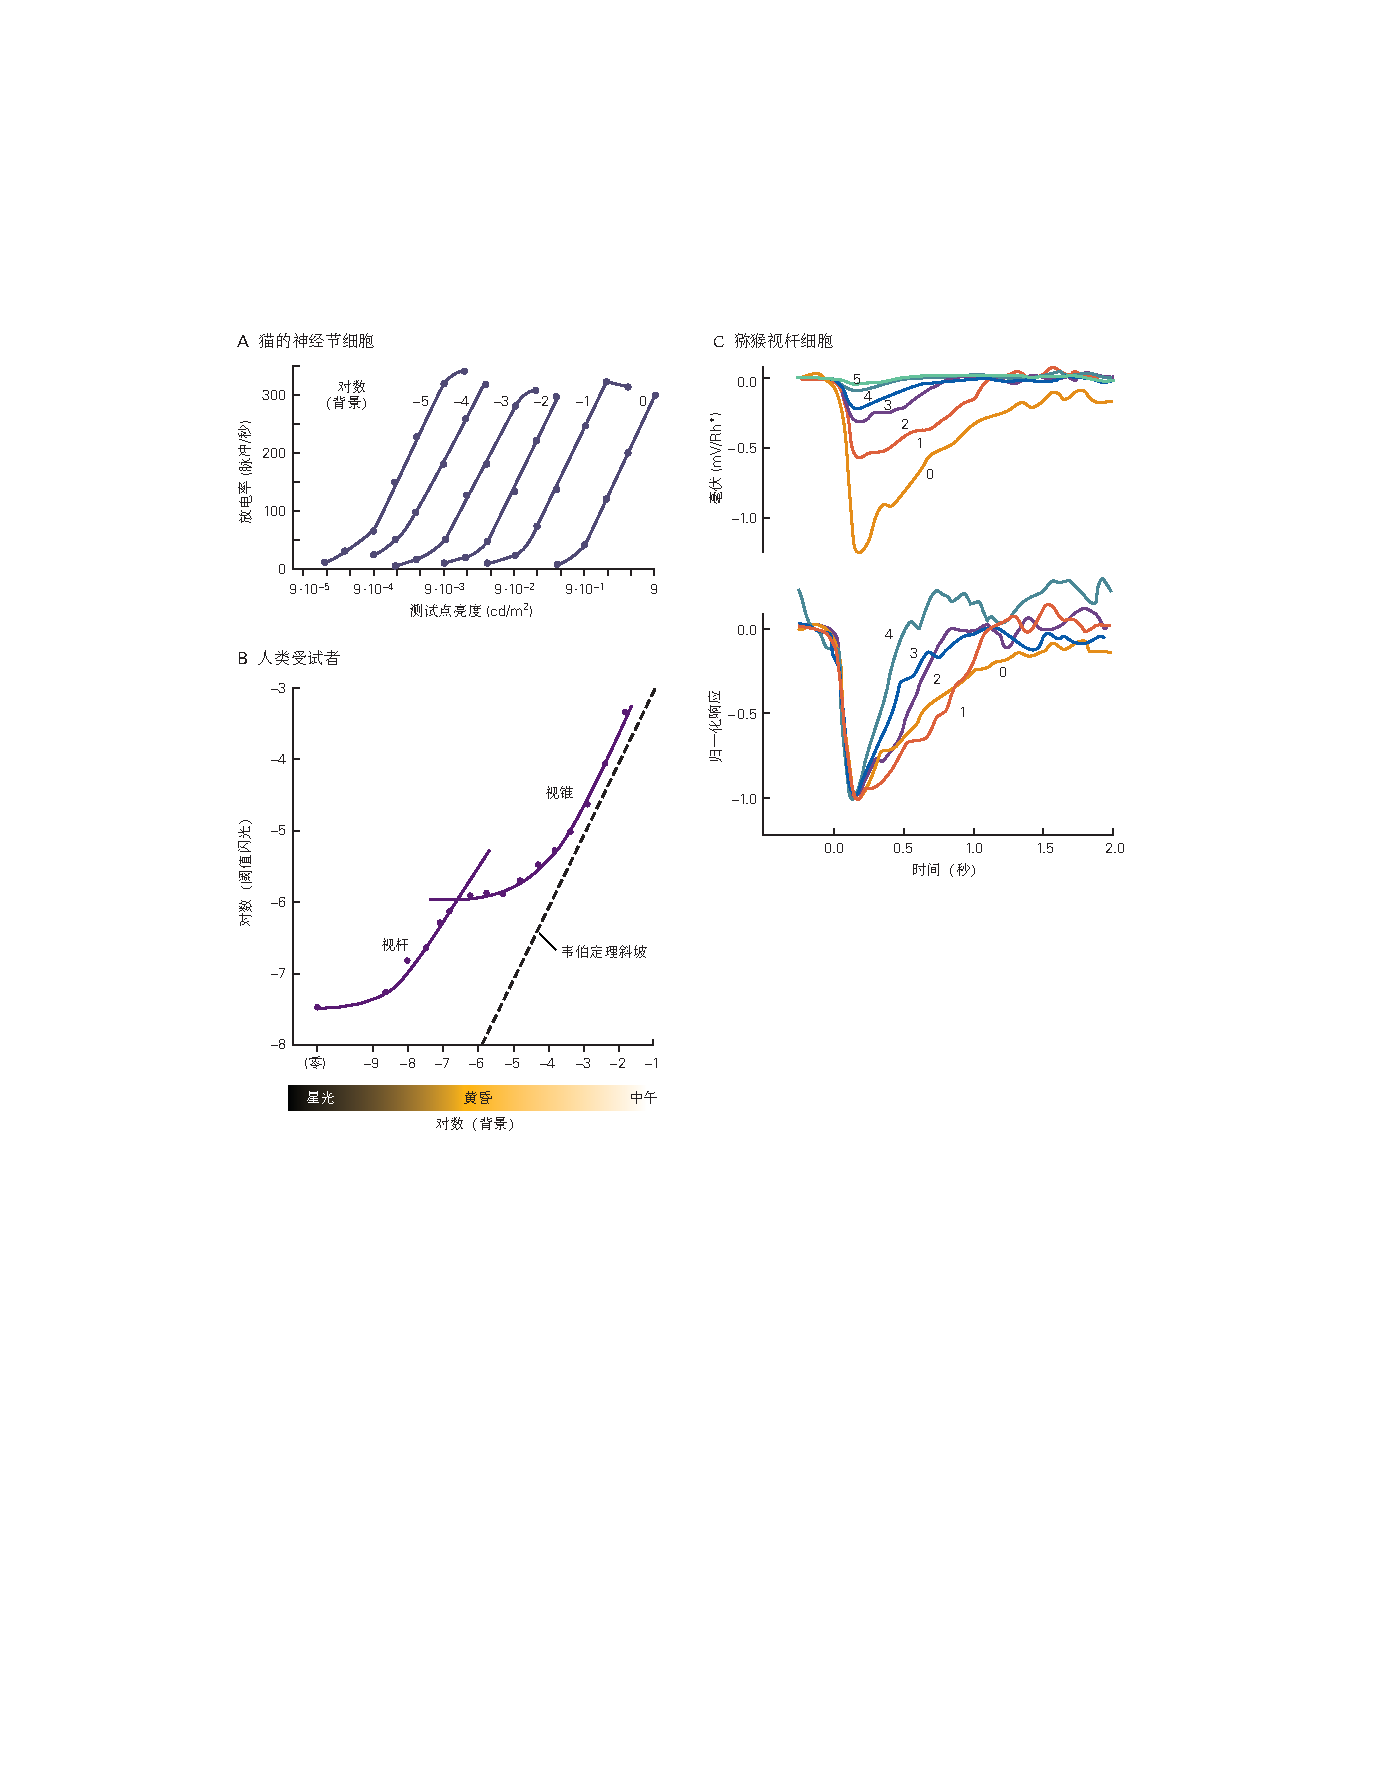
\includegraphics[width=1.0\linewidth]{chap22/fig_22_19}
	\caption{光照适应。
		A. 猫视网膜神经节细胞的感受野在稳定的背景强度下均匀照明,并在感受野中心短暂闪烁一个测试点。 
		测量闪光后的峰值激活率并根据闪光强度的对数绘制。
		每条曲线对应不同的背景强度,从左到右增加 10 倍\cite{sakmann1969scotopic}。
		B. 一个小的测试点在稳定照明的背景上短暂闪光,闪光强度逐渐增加到人类受试者刚好可以检测到的程度。
		在不同的背景强度下重复该过程。
		这里,阈值闪光强度根据背景强度绘制。
		该曲线有 2 个分支,由一个明显的扭结相连:它们对应于视杆视觉和视锥视觉的状态。
		当阈值强度与背景强度成正比时,韦伯定律的斜率表示理想化\cite{wyszecki2000color}。
		C. 上图显示了猕猴视杆细胞对不同背景强度下出现闪光的响应。
		细胞的单光子响应根据记录的膜电位除以闪光激活的\textit{视紫红质}的数量计算得出。
		单光子响应的增益随着背景强度的增加而显著降低。
		背景强度(以光子/平方微米/秒为单位)对于迹线 0 为 0,对于迹线 1 为 3.1,对于迹线 2 为 12,对于迹线 3 为 41,对于迹线 4 为 84,对于迹线 5 为 162。
		在底部图中,相同数据(最小响应除外)被归一化为相同的振幅,表明单光子响应的时间进程在高强度下加速\cite{schneeweis2000noise}。}
	\label{fig:22_19}
\end{figure}


这种增益变化对人类视觉感知的影响在心理物理学实验中显而易见。
如图~\ref{fig:22_19}B~所示,当人类受试者被要求在恒定照明的背景场中检测闪光时,在更亮的背景上检测需要更亮的闪光。
在前面讨论的理想增益控制机制下,如果 2 个刺激引起背景强度的相同分数变化,它们将产生相同的响应。
在那种情况下,阈值闪光强度应与背景强度成正比,这种关系称为韦伯适应定律,我们在考虑体细胞受体敏感性时遇到过这种关系(第~\ref{chap:chap17}~章)。
如图~\ref{fig:22_19}B~所示,视觉系统大致遵循韦伯定律:在整个视觉范围内,随着背景强度的增加,灵敏度的下降幅度有所缓和。



\subsection{多重增益控制发生在视网膜内}

光适应所需增益的巨大变化出现在视网膜内的多个部位。 
在星光下,单个视杆细胞每隔几秒就会受到一个光子的刺激,这个速度不足以改变细胞的适应状态。
然而,视网膜神经节细胞结合来自许多视杆细胞的信号,从而接收稳定的光子信号流,从而在细胞中引起光依赖性增益变化。


在稍高的光照强度下,杆状双极细胞开始适应,根据平均光照水平改变其响应能力。
接下来,我们达到单个视杆细胞的增益逐渐降低的光强度。
除此之外,视杆细胞饱和:它们所有依赖于\textit{环鸟苷-3,5-单磷酸盐}的通道都关闭了,膜电位不再对光刺激做出响应。
到这个时候,大约在黎明时分,敏感度低得多的视锥细胞得到有效刺激,并逐渐取代视杆细胞。
随着环境光进一步增加,接近中午,光适应主要来自视锥细胞内的增益变化。


光受体的细胞机制在光受体中得到了最好的理解。
前面讨论的钙依赖性反馈通路具有突出的作用。
回想一下,如图~\ref{fig:22_7}B~所示,当闪光关闭\textit{环鸟苷-3,5-单磷酸盐}门控通道时,细胞内 \ce{Ca^2+} 的减少会加速几种生化响应,从而终止对闪光的响应。
然而,如图~\ref{fig:22_19}C~所示,当光照持续时,\ce{Ca^2+} 浓度仍然很低,因此所有这些响应都处于稳定状态,既降低了增益又加速了受体对光响应的时间进程。
因此,光适应感光器可以更快地响应强度的快速变化。
这对人类视觉感知有重要影响;
如图~\ref{fig:22_14}~所示,对高频闪烁的对比敏感度随着强度的增加而增加,这也是在灵长类动物视网膜神经节细胞中观察到的效果。



\subsection{光适应改变空间处理}

除了视网膜响应的灵敏度和速度之外,光适应还改变了空间处理的规则。
如图~\ref{fig:22_10}~所示,在明亮的光线下,许多神经节细胞在它们的感受野中有一个尖锐的中心环绕结构。 
随着光线变暗,对立的环绕声变得宽广而微弱,最终消失。
在这些条件下,视网膜的回路只是简单地积累稀有光子,而不是计算局部强度梯度。
如图~\ref{fig:22_3}~所示,感受野特性的这些变化由于水平细胞和无长突细胞网络产生\textit{侧抑制}的变化而发生。
这些过程的一个重要调节剂是多巴胺,由专门的无长突细胞以依赖光的方式释放。


这些视网膜效应在人类感知上留下了印记。
在明亮的光线下,我们的视觉系统更喜欢精细的光栅而不是粗糙的光栅。
如文本框~\ref{box:22_1}~和图~\ref{fig:22_13}~所示,但在昏暗的光线下,我们对粗光栅最敏感:
随着中心环绕拮抗作用的丧失,低空间频率不再衰减。


\begin{figure}[htbp]
	\centering
	\includegraphics[width=1.0\linewidth]{chap22/fig_22_13}
	\caption{空间对比敏感度。
		A. 1. 如图 \ref{fig:22_12}~所示,人类受试者的对比敏感度使用具有不同空间频率的光栅测量。
		如图所示,在每个频率下,对比度增加到检测阈值,并且该对比度值的倒数相对于空间频率绘制。
		这些曲线是在不同的平均强度下获得的,从顶部到底部曲线减少了 10 倍\cite{de1974psychophysical}。
		2. 在高强度下测量的猕猴视网膜中 P 型神经节细胞的对比敏感度。 
		在每个空间频率下,对比度逐渐增加,直到它在神经元的放电率中产生可检测的变化。
		如 A-1 部分所示,绘制了该阈值对比度的倒数。 
		左侧的孤立点标记了零空间频率下的灵敏度,这是一个空间均匀的场\cite{derrington1984spatial}。
		B. 用正弦光栅刺激中心环绕感受野。
		神经元对视网膜上不同点的光的敏感性被建模为“高斯差分”感受野,其中兴奋性中心为窄正高斯分布,抑制性周围为宽的负高斯分布。
		将光栅刺激的轮廓(强度与位置)与感受野的轮廓(灵敏度与位置)相乘,并在所有空间上积分,计算出特定光栅传递的刺激强度。
		右图显示了感受野对不同频率光栅的灵敏度。
		在低空间频率下,环绕声的负贡献抵消了中心的贡献,导致差异曲线下降\cite{enroth1984functional}。}
	\label{fig:22_13}
\end{figure}


\begin{figure}[htbp]
	\centering
	\includegraphics[width=0.83\linewidth]{chap22/fig_22_12}
	\caption{正弦波光栅显示器用于人类受试者的心理物理学实验。
		在图~\ref{fig:22_13}~中讨论的实验中使用了此类刺激。}
	\label{fig:22_12}
\end{figure}


总之,光照适应有 2 个重要作用。
一种是丢弃有关环境光强度的信息,同时保留有关物体反射率的信息。
另一个是将视网膜神经节细胞中的小动态放电范围与环境中的大范围光强度相匹配。
这些大的增益变化必须在视神经纤维中产生动作电位之前通过分级神经元信号来完成,因为这些纤维的放电率只能在 2 个数量级内有效变化。
事实上,光适应的关键需求可能就是为什么这种神经回路位于眼睛而不是视神经另一端的大脑中。



\section{亮点}

1. 视网膜将投射到光受体上的光模式转化为神经信号,这些信号通过视神经传送到大脑中专门的视觉中心。 
不同的神经节细胞群沿着并行通路传输视网膜图像的多种神经表征。


2. 视网膜丢弃了受体水平上可用的大部分刺激信息,并提取了对中央视觉系统有用的视野的某些低层特征。
精细的空间分辨率仅在凝视中心的狭窄区域中保持。
图像中的强度梯度(例如物体边缘)在空间均匀的部分上得到强调;
场景的不变部分增强了时间变化。


3. 视网膜能灵活适应视觉条件的变化,尤其是昼夜光照变化较大。
关于绝对光照水平的信息大部分被丢弃,有利于随后对场景内物体反射率的分析。 


4. 当色素分子吸收光子时,光刺激的转导开始于感光细胞的外段。
这启动了一个放大的 G 蛋白级联响应,最终降低了膜电导,使光受体超极化,并减少了突触处的谷氨酸释放。 
多种反馈机制(其中细胞内 \ce{Ca^2+} 具有重要作用)用于关闭级联中的酶并终止光响应。


5. 杆状感光器是高效的光收集器并服务于夜间视觉。
视锥细胞的敏感性要低得多,并且全天都在发挥作用。
视锥突触到双极细胞上,进而激发神经节细胞。
视杆连接到专门的视杆双极细胞,其信号通过无长突细胞传递到视锥双极细胞。 


6. 垂直兴奋通路由主要是抑制性的水平连接调节。
通过这些横向网络,神经节细胞感受野周围的光抵消了中心光的影响。
同样的负反馈回路也加强了神经节细胞的瞬态响应。


7. 将信息隔离到并行通路中以及通过抑制性横向连接形成响应特性是视觉系统中普遍存在的组织原则。


